% \chapter{DISPLACEMENT OF SKEWED BRIDGE}
\chapter{斜交桥梁的位移}
% This appendix provides summary of the work for addressing the effect of skew on lateral movement of the bridge at the abutment.
本附录提供了解决斜交对桥台处桥梁横向移动影响的工作总结。

% \section{BACKGROUND}
\section{背景}
% A skewed bridge is a bridge with the longitudinal axis at an angle other than 90° with the piers and abutments. The skew angle, θ, is shown in Figure B.1. With skewed integral abutment bridges, the soil passive pressure developed in response to thermal elongation has a component in the transverse direction as illustrated in Figure B.1. Within certain limits of the skew angle, soil friction on the abutment will resist the transverse component of passive pressure. However, if the soil friction is insufficient, then, depending on the transverse stiffness of the abutment, either significant transverse forces or significant transverse movements could be generated.
斜桥是纵轴与桥墩和桥台呈非 \qty{90}{\degree} 角度的桥梁。 斜交角 $\theta$ 如\cref{fig:skewed-bridge-thermal-elongation} 所示。对于斜交的整体式桥台桥,在温度作用下产生的台背土被动压力在横向方向上有一个分量,如\cref{fig:skewed-bridge-thermal-elongation} 所示。 在一定的斜交角范围内,桥台上的土壤摩擦力将抵抗被动压力的横向分量。 然而,如果土壤摩擦力不足,则根据桥台的横向刚度,可能会产生显著的横向力或显著的横向运动。

\begin{figure}
  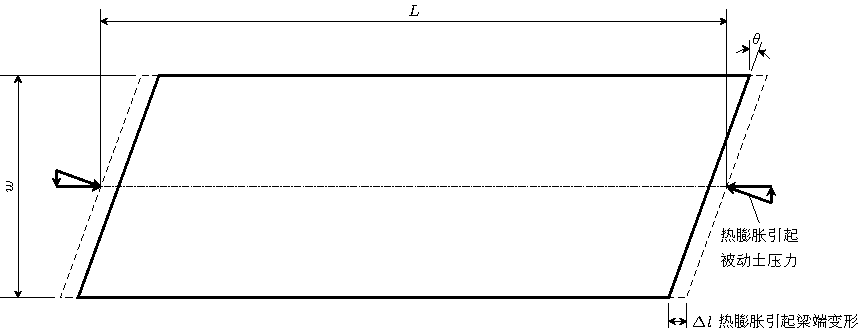
\includegraphics{skewed-bridge-thermal-elongation.pdf}
  % \caption{Components of abutment soil passive pressure response to thermal elongation in skewed integral abutment bridges}
  \caption{斜交整体式桥台在温度作用下产生的桥台土被动压力分量}
  \label{fig:skewed-bridge-thermal-elongation} 
\end{figure}

% \cref{fig:two-span-skewed-bridge} shows a two-span bridge with a skew angle of \ang{45} (Nicholson et al. 1997). This bridge was constructed in 1969 with semi-integral abutments. The semi-integral construction included an integral end diaphragm that was designed to move with the superstructure which slides longitudinally, and is guided transversely by, relatively stiff abutments.
\cref{fig:two-span-skewed-bridge} 显示了一个斜交角为 \ang{45} 的双跨桥(Nicholson 等人,1997 年)。 这座桥建于 1969 年,采用半整体式桥台。 半整体式结构包括一个整体式端隔板,设计用于与纵向滑动的上部结构一起移动,并由相对坚硬的桥台横向引导。

\begin{figure}
  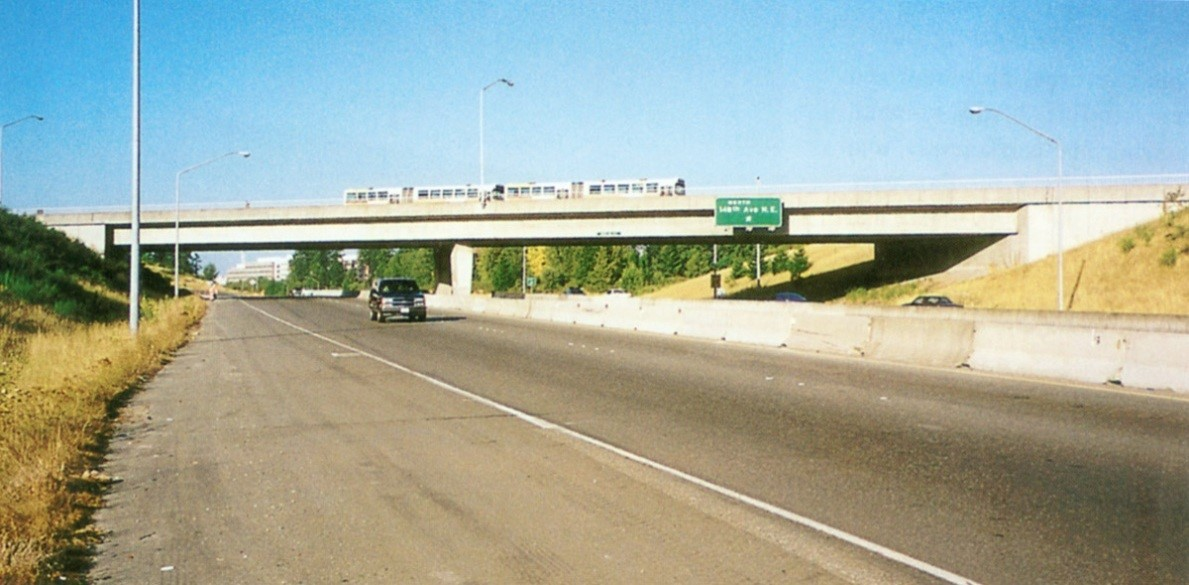
\includegraphics[width=0.8\linewidth]{two-span-skewed-bridge.jpg}
  % \caption{Two-span semi-integral abutment bridge with an overall length of 89 m (259 ft), width of 11.6 m (38 ft), and a skew angle of 45°. (Nicholson et al. 1997)}
  \caption{两跨半整体式桥台,总长度为 \qty{89}{m},宽度为 \qty{11.6}{m},斜交角为 \ang{45}}
  \label{fig:two-span-skewed-bridge}
\end{figure}

% \cref{fig:cracking-abutment-wall} shows cracking in the abutment wall near an acute corner of the superstructure, presumably caused by transverse forces related to soil pressures.
\cref{fig:cracking-abutment-wall} 显示了上部结构锐角附近的桥台背墙开裂,这可能是由与土压力相关的横向力导致。
% \cref{fig:asphalt-overlay-distress} shows distress in an asphalt overlay at the skewed end of an approach slab because of the transverse movement (Tabatabai et al. 2005).
\cref{fig:asphalt-overlay-distress} 显示了由于横向运动导致引道板倾斜端的沥青覆盖层的损坏(Tabatabai 等人,2005 年)。

\begin{figure}
  \begin{minipage}{0.5\linewidth}\centering
    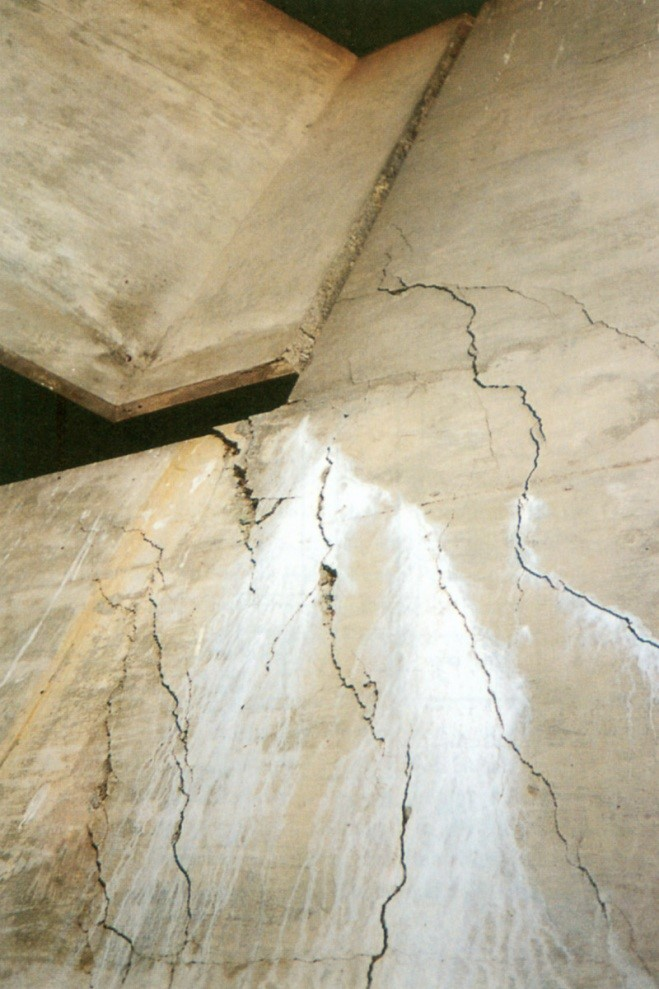
\includegraphics[height=8cm]{cracking-abutment-wall.jpg}
    % \caption{Cracking in the abutment wall near an acute corner of the superstructure for the bridge shown in \cref{fig:two-span-skewed-bridge}. (Nicholson et al. 1997)}
    \caption{上部结构锐角附近的桥台墙开裂}
    \label{fig:cracking-abutment-wall}
  \end{minipage}%
  \begin{minipage}{0.5\linewidth}\centering
    
\includegraphics[height=8cm]{asphalt-overlay-distress.jpg}
    % \caption{Asphalt overlay distress (west end). (Tabatabai et al. 2005)}
    \caption{沥青覆盖层损坏(西侧)}
    \label{fig:asphalt-overlay-distress}
  \end{minipage}
\end{figure}

% \cref{fig:barrier-distress} shows a closer view of the barrier wall joint from \cref{fig:asphalt-overlay-distress} at the end of the approach slab. The expansion joint in the barrier wall was made perpendicular to the longitudinal direction and could not accommodate the transverse movement.
\cref{fig:barrier-distress} 显示了引道板末端 \cref{fig:asphalt-overlay-distress} 的屏障墙接缝的近距离视图。 隔离墙中的伸缩缝垂直于纵向,不能适应横向移动。

\begin{figure}
  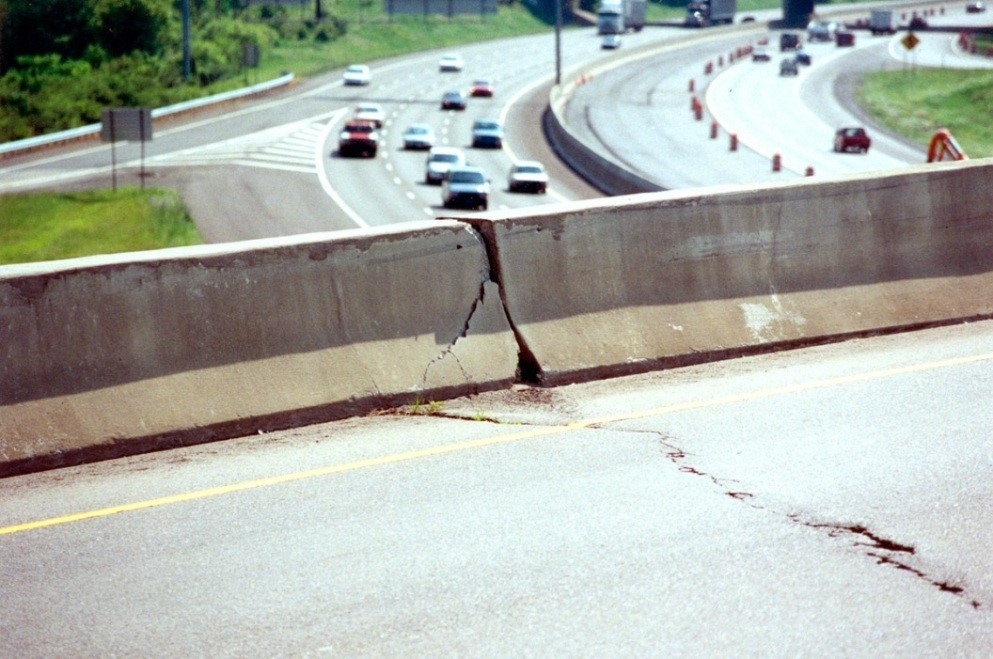
\includegraphics[width=0.8\linewidth]{barrier-distress.jpg}
  % \caption{Barrier distress at west abutment. (Tabatabai et al. 2005)}
  \caption{西桥台护栏损坏}
  \label{fig:barrier-distress}
\end{figure}

% Because of potential problems and uncertainty related to the response of skewed integral abutments, many State DOTs limit the skew angle. A typical limit for maximum skew angle for integral abutment bridges used by many States is 30 degrees. However, maximum skew angle limits in various States range from 0 degrees to no limit (Chandra 1995). Therefore studies were conducted in the FHWA Jointless Bridge Project (Oesterle and Lotfi 2005) to:
由于与倾斜整体基台的响应相关的潜在问题和不确定性,许多州\acrlong*{dot}限制了倾斜角度。 许多国家使用的整体式桥台桥的最大倾斜角的典型限制是 \ang{30}。 但是,各个州的最大倾斜角限制范围从 \ang{0} 到无限制(Chandra 1995)。 因此,在 \acrshort*{fhwa} 无缝桥项目(Oesterle 和 Lotfi 2005)中进行了以下研究:

% \begin{enumerate}
%   \item Develop a relationship between skew angle and abutment soil friction for limiting skew.
%   \item Develop a relationship for the magnitude of forces required to restrain transverse movement in integral abutment bridges with large skew angles.
%   \item Develop a relationship between skew angle and expected transverse movement for a typical integral stub abutment with no special design features to restrain this movement.
%   \item Compare analytical results with field data for a skewed bridge that was monitored as part of the experimental portion of this project.
%   \item Perform a sensitivity study to demonstrate the relationship between transverse movement and longitudinal expansion for various skew angles and ratios of bridge length to width.
% \end{enumerate}
\begin{enumerate}
  \item 建立倾斜角度和基台土摩擦力之间的关系以限制倾斜。
  \item 建立约束大斜角整体式桥台横向移动所需力大小的关系。
  \item 对于没有特殊设计特征来限制这种运动的典型整体式短端基台,建立倾斜角与预期横向运动之间的关系。
  \item 将分析结果与作为该项目实验部分的一部分进行监测的斜桥的现场数据进行比较。
  \item 进行敏感性研究,以证明各种倾斜角度和桥梁长宽比的横向移动和纵向扩展之间的关系。
\end{enumerate}

% This work was accomplished by developing equilibrium and compatibility equations for end abutment forces and, for the case of a typical stub abutment, solving these relationships for various skew angles and bridge length-towidth ratios.
这项工作是通过开发端部基台力的平衡和相容性方程来完成的,对于典型的短端基台,解决了各种倾斜角度和桥梁长宽比的这些关系。

% \section{ANALYSES FOR TRANSVERSE RESPONSE TO THERMAL EXPANSION}
\section{热膨胀的横向响应分析}
% \subsection{Skew Angle Limit for Limiting Transverse Effects}
\subsection{限制横向影响的极限斜交角度}
% \cref{fig:soil-pressure-abutment-friction} shows the passive soil pressure response, $P_\text{p}$ , due to thermal expansion and soil/abutment interface friction, $F_\text{af}$ , assuming no rotation in the plane of the bridge superstructure. For rotational equilibrium:
\cref{fig:soil-pressure-abutment-friction} 显示被动土压力响应 $P_\text{p}$ ,由于热膨胀和土壤/桥台界面摩擦 $F_\text{af}$ ,假设桥梁上部结构平面内无旋转。 由转动平衡关系有:
\begin{equation}
  \label{eq:soil-pressure-vs-friction-1}
  F_\text{af} (L\cos\theta)= P_\text{p} (L\sin\theta)
\end{equation}
在土于混凝土之间的界面上,
\begin{equation}
  \label{eq:soil-pressure-vs-friction-2}
  F_\text{af} = P_\text{p} \tan \delta
\end{equation}
\begin{EqDesc}{\tan\delta}
  \item [\tan\delta] 成型混凝土与土界面的摩擦系数。
\end{EqDesc}

% Substituting \cref{eq:soil-pressure-vs-friction-1} into \cref{eq:soil-pressure-vs-friction-2}:
将 \cref{eq:soil-pressure-vs-friction-1} 代入 \cref{eq:soil-pressure-vs-friction-2}中:
\begin{gather}
  \tan \delta =\frac{\sin \theta}{\cos \theta} = \tan \theta \qquad \text{或} \\
  \delta = \theta \notag
\end{gather}

% Therefore, the bridge superstructure can be held in rotational equilibrium until the skew angle exceeds the angle of interface friction. Integral abutments are typically backfilled with granular material. NCHRP Report 343 lists a friction angle of \ang{22} to \ang{26} for formed concrete against clean gravel, gravel sand mixtures, and wellgraded rock fill (Arsoy et al. 2002). Based on these data, the angle of $\theta = \ang{20}$ represents a reasonably conservative skew angle limit below which special considerations for transverse forces or transverse movement are not needed.
因此,桥梁上部结构可以保持旋转平衡,直到倾斜角超过界面摩擦角。整体式桥台通常用颗粒材料回填。 NCHRP 报告 343 列出了成型混凝土与清洁砾石、砾石砂混合物和分级良好的岩石填充物的摩擦角为 \ang{22} 至 \ang{26}(Arsoy 等人,2002 年)。 根据这些数据,$\theta = \ang{20}$ 的角度代表一个合理保守的倾斜角度限制,低于该限制时不需要对横向力或横向移动进行特殊考虑。


\begin{figure}
  % \includegraphics[width=\linewidth]{graphic-file}
  % \caption{Soil pressure load, Pp, and soil abutment interface friction, Faf.}
  \caption{Soil pressure load, $P_\text{p}$, and soil abutment interface friction, $F_\text{af}$.}
  \label{fig:soil-pressure-abutment-friction}
\end{figure}

% With larger skew angles, the integral abutment can be either designed to resist the transverse force generated by the soil passive pressure in an attempt to guide the abutment movement to be predominantly longitudinal, or detailed to accommodate the transverse movement.
对于较大的斜交角,整体式基台可以设计为抵抗土壤被动压力产生的横向力,以试图引导桥台主要纵向运动,或者详细设计以适应横向运动。

% \subsection{Forces Required to Resist Transverse Movement}
\subsection{Forces Required to Resist Transverse Movement}
Adding lateral resistance of the abutment, $F_\text{a}$ , to wall/soil interface friction, $F_\text{af}$ ., in {fig:soil-pressure-abutment-friction}, rotational equilibrium is found by:
\begin{equation}
  \label{eq:rotational-equilibrium}
  (F_\text{a} + F_\text{af})(L \cos\theta)= P_\text{p} (L \sin\theta)
\end{equation}
Substituting from \cref{eq:soil-pressure-vs-friction-2} into \cref{eq:rotational-equilibrium}:
\begin{equation}
  F_\text{a} = P_\text{p} (\tan\theta - \tan\delta)
\end{equation}

$F_\text{a}$ is the summation of abutment lateral resistance from pile and passive pressure on the substructure surface perpendicular to the abutment.

\cref{fig:pp-vs-fa} shows the relationship between Fa and $P_\text{p}$ , assuming the interface friction angle, $\delta$ , to be \ang{20}. As shown in \cref{fig:pp-vs-fa}, the force required to resist transverse movement is a significant portion of the soil passive pressure, $P_\text{p}$ . It should be noted that $P_\text{p}$ is not necessarily full passive pressure, but can be determined for the end movement using relationships calculated by Clough and Duncan (Clough and Duncan 1991; Barker et al. 1991) shown in {fig:soil-pressure-abutment-friction}. The end movement to consider in calculating passive pressure is the end movement normal to the abutment, $\Delta l_\text{n}$ .


\begin{figure}
  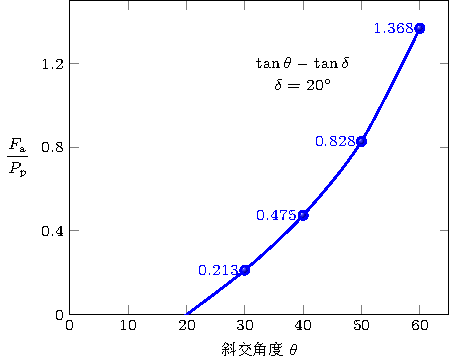
\includegraphics{pp-vs-fa.pdf}
  % \caption{Relationship between force required for abutment lateral resistance, $F_\text{a}$, and passive pressure response, $P_\text{p}$, to restrain lateral movement.}
  \caption{Relationship between force required for abutment lateral resistance, $F_\text{a}$, and passive pressure response, $P_\text{p}$, to restrain lateral movement.}
  \label{fig:pp-vs-fa}
\end{figure}

As illustrated in Figure B.8, this end movement is:
\begin{equation}
  \Delta l_\text{n} =  \Delta l \cos\theta
\end{equation}
\begin{EqDesc}{\Delta l}
  \item[\Delta l] maximum expected end movement for thermal re-expansion from the starting point of full contraction for the full range of effective bridge temperatures as discussed in Section 8.6.2.3.1.
\end{EqDesc}


From \cref{fig:delataln-delatal}, it can be seen that $\Delta l_\text{n}$ is reduced with respect to $\Delta l$ as the skew angle, $\theta$, increases. This relationship helps offset the increase in $F_\text{a}/P_\text{p}$ with increasing $\theta$. However, $F_\text{a}$ will still be a sizeable portion of $P_\text{p}$.

\begin{figure}
  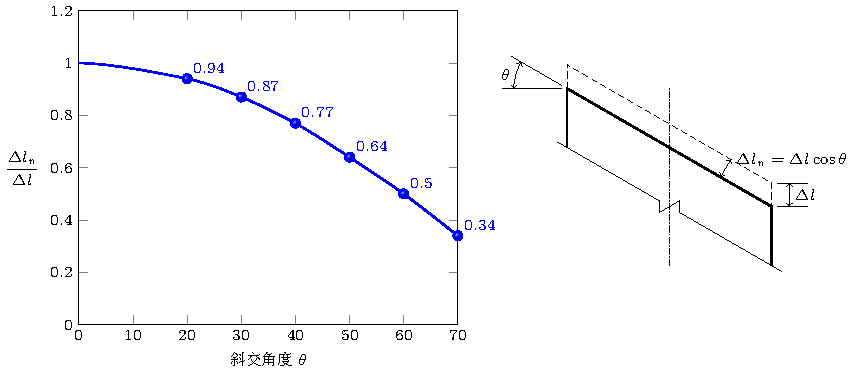
\includegraphics{delataln-delatal.pdf}
  % \caption{Relationship between end normal movement, $\Delta l_\text{n}$, and end thermal expansion, $\Delta l$.}
  \caption{Relationship between end normal movement, $\Delta l_\text{n}$, and end thermal expansion, $\Delta l$.}
  \label{fig:delataln-delatal}
\end{figure}

For relatively short bridges and/or bridges in locations with small effective temperature ranges, it may be feasible to design the abutment substructure to resist $F_\text{a}$. However, it should be understood that for whatever means used to develop $F_\text{a}$ (battered pile and/or lateral passive soil resistance), lateral movements are required to develop the resistance. Therefore, details anticipating some transverse movement should be used. The expected movements are a function of the relative stiffnesses of response for $P_\text{p}$ and $F_\text{a}$. It should also be noted that adding battered piles to an integral abutment for lateral loading will also increase the stiffness in the longitudinal direction, which induces more demand on the superstructure and connections between the girders and abutments.

% \section{EXPECTED TRANSVERSE MOVEMENT WITH TYPICAL INTEGRAL ABUTMENT}
\section{典型整体基台的预期横向移动}
% \subsection{Method of Analyses}
\subsection{分析方法}
To investigate the relationship between skew angle and expected transverse movement for a typical integral stub abutment, a set of relationships were derived based on equilibrium and compatibility of end abutment forces in the plane of the bridge superstructure. For this analysis, the superstructure is assumed to act as a rigid body with rotation, $\beta$, about the center of the deck (for a longitudinally symmetrical bridge). The rotation occurs to accommodate the thermal end movement, $\Delta l$ . Forces considered in response to this movement include soil pressure on the abutment and wingwalls, wall/soil interface friction on the abutment, and pile forces normal to and in line with the abutment and wingwalls. Details of the forces, stiffness, and equations of compatibility and equilibrium are provided in the report on the analytical work for the FHWA Jointless Bridge Project (Oesterle 2005).

A spreadsheet program was used for solving rotational equilibrium in the plane of the deck. For a given end thermal movement, $\Delta l$ , the equilibrium position can be found using an iterative analysis by progressively increasing the rotation angle, $\beta$ , until the sum of the in-plane moments is zero.

% \subsection{Results of Analyses for Instrumented Bridge}
\subsection{整体式桥梁的分析结果}
As part of the experimental program for the Jointless Bridge Project (Tabatabai et al. 2005), a heavily skewed bridge in Tennessee was instrumented and monitored for one year. This bridge carries U.S. Interstate 40 (I-40) over Ramp 2B in Knox County, Tennessee. It has a three-span steel plate girder superstructure with an overall length of 415.92 ft and integral abutments. This structure is sharply skewed with a skew angle of 59.09º. The three span lengths are 139.83 ft, 208 ft, and 68.08 ft. The bridge was instrumented to monitor the longitudinal and transverse movements of the east abutment, and obtain an indication of restraint to the longitudinal expansion.

The east abutment was analyzed using the spreadsheet program developed to solve for rotational equilibrium (Oesterle 2005; Oesterle and Lotfi 2005). Based on the experimental data, an end movement of Δl = 0.781 in. was used in the analysis. A measured superstructure rotation angle of β = 0.000224 radians corresponded with the Δl = 0.781 in. Using the spreadsheet to determine rotational equilibrium, an angle of β = 0.000226 radians was calculated. The calculated value indicated very good agreement with the measured data.

% \subsection{Sensitivity Analyses for the Effects of Skew Angle on Transverse Movement and Longitudinal Restraint}
\subsection{斜交角对横向运动和纵向约束影响的敏感性分析}
To demonstrate the effects of skew angle on expected transverse movement and longitudinal restraint forces,
further analyses were carried out using the spreadsheet program. Variables included skew angle and the length-towidth
ratio for the bridge. The abutment for the instrumented bridge is a relatively typical type of stub abutment used
in Tennessee and was used as the baseline abutment for the analyses (Oesterle 2005; Oesterle and Lotfi 2005).

The instrumented bridge is relatively wide compared to the length. The ratio of length to width (L/W) for this
bridge is 3.15. To demonstrate the sensitivity to the bridge L/W ratio, the analyses were repeated for abutments
reduced to 2/3W and 1/3W. The length of the wingwalls at each skew angle was kept constant.

Results of these analyses for the ratio of transverse movement to longitudinal movement, t1 l
Δ
Δ are shown in
Figure B.9 for a Δl of 1 in. The transverse movement, t1 Δ , is the transverse movement of the acute corner of the
bridge deck. This is the corner that experiences the greatest transverse movement because of the skew angle.

The results in \cref{fig:transverse-movement-thermal-expansion} demonstrate the increase in the transverse movement with increasing skew angle. The
data in \cref{fig:transverse-movement-thermal-expansion} also demonstrates the increase in transverse movement with decreasing L/W ratio. It should be
pointed out that the change in L/W was accomplished in the analyses by decreasing the width and keeping the length
constant. The length of the wingwall at each skew angle was constant; therefore, the results in \cref{fig:transverse-movement-thermal-expansion}
demonstrate the effects of increasing the ratio of the length of the wingwalls to the length of the abutment wall. The
data in \cref{fig:transverse-movement-thermal-expansion} shows that increasing the wingwall length relative to the abutment wall length (which includes
increasing the number of wingwall piles relative to the number of abutment wall piles) can significantly decrease the
transverse movement. However, the wingwalls and abutment must be designed to transmit the wingwall forces into
the superstructure.

\begin{figure}
  % \includegraphics[width=\linewidth]{graphic-file}
  % \caption{Relationship between transverse movement at the acute corner, Δt1, and thermal expansion, Δ, for an expansion of 1 in. with constant length bridge, L = 415.92 ft, and varying L/W.}
  \caption{Relationship between transverse movement at the acute corner, Δt1, and thermal expansion, Δ, for an expansion of 1 in. with constant length bridge, L = 415.92 ft, and varying L/W.}
  \label{fig:transverse-movement-thermal-expansion}
\end{figure}

\cref{fig:restraint-force-skew-angle} shows the resulting total longitudinal restraint force for these analyses and demonstrates the decrease in longitudinal restraint with increasing skew angle. For the full-width bridge with L/W = 3.15, the longitudinal restraint at a skew angle of θ = 60 degrees is approximately 60\% of the longitudinal restraint at θ = 25 degrees. For the larger L/W = 9.45, the ratio of longitudinal restraint at θ = 60 degrees is approximately 70 percent of the restraint at θ = 25 degrees. This demonstrates the increase in restraint resulting from the increase in resistance to lateral moment because of the larger ratio of wingwall length to abutment length.

\begin{figure}
  % \includegraphics[width=\linewidth]{graphic-file}
  % \caption{Relationship between resultant longitudinal restraint force and skew angle for thermal expansion, Δ, of 1 in. with constant length bridge, L = 415.92 ft, and varying L/W.}
  \caption{Relationship between resultant longitudinal restraint force and skew angle for thermal expansion, Δ, of 1 in. with constant length bridge, L = 415.92 ft, and varying L/W.}
  \label{fig:restraint-force-skew-angle}
\end{figure}

% \subsection{Design Recommendations}
\subsection{设计建议}
Since the baseline abutment used in these analyses is a relatively typical stub abutment (but also relatively deep, with an abutment height of 13.0 ft and with strong axis pile bending for movement normal to the abutment versus weak axis bending for movement parallel to the abutment), the data in \cref{fig:transverse-movement-thermal-expansion} represents a reasonably large estimate for the transverse movement of skewed abutments. Although there is significant uncertainty for actual soil and pile stiffness, the maximum expected end movement, Δl , discussed in Section 8.6.2.3.1 includes a multiplier to account for uncertainty. Therefore, it is suggested that the data in \cref{fig:transverse-movement-thermal-expansion} can be used by designers to determine an approximate estimate for expected transverse movement in skewed integral abutments resulting from the restraint of longitudinal thermal expansion. In addition, the relationships between longitudinal restraint force and skew angle shown in \cref{fig:restraint-force-skew-angle} can be used to estimate the relative decrease in restraint forces in a skewed bridge. Also, the transverse movements can be used to estimate the transverse forces on the wingwall resulting from passive soil load and pile, and to estimate longitudinal and transverse movement for the abutment pile for biaxial bending considerations. All of the other components of movement and forces can be determined from Δt1 and Δl using equations presented in the full analytical report (Oesterle 2005).
